%% LyX 2.0.6 created this file.  For more info, see http://www.lyx.org/.
%% Do not edit unless you really know what you are doing.
\documentclass[english]{article}
\usepackage[T1]{fontenc}
\usepackage[latin9]{inputenc}
\usepackage{geometry}
\geometry{verbose,tmargin=1in,bmargin=1in,lmargin=1in,rmargin=1in}
\usepackage{amsmath}
\usepackage{graphicx}

\makeatletter

%%%%%%%%%%%%%%%%%%%%%%%%%%%%%% LyX specific LaTeX commands.
%% Because html converters don't know tabularnewline
\providecommand{\tabularnewline}{\\}

\@ifundefined{showcaptionsetup}{}{%
 \PassOptionsToPackage{caption=false}{subfig}}
\usepackage{subfig}
\makeatother

\usepackage{babel}
\begin{document}

\title{Pattern Classification and Machine Learning:\\
Project Report}


\author{Nicolas Voirol (186268), Damien Firmenich(178474)\\
EPFL, School of Computer and Communication Sciences}


\date{Spring 2013}

\maketitle

\section{Introduction}

Pattern classification and machine learning provide us with a large
set of powerful tools and techniques. The sheer number and the diversity
of these tools can make selecting the ideal technique for a given
problem quite difficult. We could simply decide we want to use the
best techniques available to make sure our system is optimal, but
with complexity comes time consumption. Therefore, when using an elaborate
tool to solve a classification problem, it is generally useful to
make sure it actually performs better than a simpler technique. This
project compares the Multi-Layer Perceptron technique against Least
Squares Estimation and Logistic Regression on the NORB dataset.


\section*{Methods}

The theory places gradient descent in batch mode above stochastic
online descent in terms of the optimality of each update. We therefore
implemented partial (or mini) batch mode with varying batch size to
compare their actual impact on convergence speed and final error rate.
We implemented this feature in our MLP and Logistic Regression classifiers
since they are both based on gradient descent.


\subsection*{Model and parameters}


\subsection{Binary MLP and multi-way MLP}


\paragraph{Backpropagation}

The vectorized backpropagation equations that we implemented for the
binary MLP are as follows :

\begin{eqnarray*}
\mathbf{r}^{\left(3\right)}=\sigma\left(\mathbf{a}^{\left(3\right)}\right)-\frac{1}{2}\left(\mathbf{t}+1\right) & \Rightarrow & \nabla_{\mathbf{w}^{\left(3\right)}}E_{i}=r^{\left(3\right)}\left(z^{\left(2\right)}\right)^{T}\\
\mathbf{r}_{L}^{\left(2\right)}=\mathbf{a}_{LR}^{\left(2\right)}\sigma'\left(\mathbf{a}_{L}^{\left(2\right)}\right)\sigma\left(\mathbf{a}_{R}^{\left(2\right)}\right)\mathbf{w}^{\left(3\right)}\mathbf{r}^{\left(3\right)} & \Rightarrow & \nabla_{\mathbf{w}_{L}^{\left(2\right)}}E_{i}=\mathbf{r}_{L}^{\left(2\right)}\left(\mathbf{z}_{L}^{\left(1\right)}\right)^{T}\\
\mathbf{r}_{R}^{\left(2\right)}=\mathbf{a}_{LR}^{\left(2\right)}\sigma\left(\mathbf{a}_{L}^{\left(2\right)}\right)\sigma'\left(\mathbf{a}_{R}^{\left(2\right)}\right)\mathbf{w}^{\left(3\right)}\mathbf{r}^{\left(3\right)} & \Rightarrow & \mathbf{\nabla}_{\mathbf{w}_{R}^{\left(2\right)}}E_{i}=\mathbf{r}_{R}^{\left(2\right)}\left(\mathbf{z}_{R}^{\left(1\right)}\right)^{T}\\
\mathbf{r}_{LR}^{\left(3\right)}=\sigma\left(\mathbf{a}_{L}^{\left(2\right)}\right)\sigma\left(\mathbf{a}_{R}^{\left(2\right)}\right)\mathbf{w}^{\left(3\right)}\mathbf{r}^{\left(3\right)} & \Rightarrow & \mathbf{\nabla}_{\mathbf{w}_{LR}^{\left(2\right)}}E_{i}=\mathbf{r}_{LR}^{\left(2\right)}\left[\mathbf{z}_{L}^{\left(1\right)}\,\mathbf{z}_{R}^{\left(1\right)}\right]^{T}\\
\mathbf{r}_{L}^{\left(1\right)}=\left(\textrm{diag}\, g'\left(\mathbf{a}_{L}^{\left(2\right)}\right)\right)\left(\left(\mathbf{w}_{L}^{\left(2\right)}\right)^{T}\mathbf{r}_{L}^{\left(2\right)}+\left(\mathbf{w}_{LR[L]}^{\left(2\right)}\right)^{T}\mathbf{r}_{LR}^{\left(2\right)}\right) & \Rightarrow & \mathbf{\nabla}_{\mathbf{w}_{L}^{\left(1\right)}}E_{i}=\mathbf{r}_{L}^{\left(1\right)}\left(\mathbf{x}_{L}\right)^{T}\\
\mathbf{r}_{R}^{\left(1\right)}=\left(\textrm{diag}\, g'\left(\mathbf{a}_{R}^{\left(2\right)}\right)\right)\left(\left(\mathbf{w}_{L}^{\left(2\right)}\right)^{T}\mathbf{r}_{L}^{\left(2\right)}+\left(\mathbf{w}_{LR[R]}^{\left(2\right)}\right)^{T}\mathbf{r}_{LR}^{\left(2\right)}\right) & \Rightarrow & \mathbf{\nabla}_{\mathbf{w}_{R}^{\left(1\right)}}E_{i}=\mathbf{r_{R}^{\left(1\right)}}\left(\mathbf{x}_{R}\right)^{T}
\end{eqnarray*}


\begin{tabular}{|c|l|}
\hline 
Notation & Description\tabularnewline
\hline 
\hline 
$\mathbf{w}_{LR[L]}^{\left(2\right)}$, $\mathbf{w}_{LR[R]}^{\left(2\right)}$  & portion of the weight matrix corresponding to the left, respectively
right, image\tabularnewline
\hline 
$g\left(\cdot\right)$ & transfer function $tanh\left(\cdot\right)$\tabularnewline
\hline 
$\left[\mathbf{z}_{L}^{\left(1\right)}\,\mathbf{z}_{R}^{\left(1\right)}\right]$ & concatenation of $\mathbf{z}_{L}^{\left(1\right)}$ and $\mathbf{z}_{R}^{\left(1\right)}$.\tabularnewline
\hline 
\end{tabular}

\smallskip{}


The residuals are computed using the derivative of the $tanh$ transfer
function, and the derivative of the logistic loss function. Then the
gradients at each layer and for each stereo image (left, right) are
computed using the residuals.


\paragraph{Multi-way classification}

Most of the MLP we implemented for binary classification could be
reused for multi-way classification. Only two changes were necessary
:
\begin{enumerate}
\item The computation of the error on the top-layer had to be modified to
squared error on \emph{1 of K} coded target vector \textbf{\emph{t}},
which implied the following change to the top-layer residual :
\[
\mathbf{r}^{\left(3\right)}=\mathbf{a}^{\left(3\right)}-\mathbf{\tilde{t}}
\]

\item Since we now have 5 outputs instead of a single one, the computation
of the class associated with the input image is becomes $\underset{i=1,...,5}{argmax}\left(\mathbf{a}_{i}^{\left(3\right)}\right)$
instead of $sign\left(a^{\left(3\right)}\right)$.
\end{enumerate}
Interestingly, the equations for backpropagation don't need to be
changed as they are vectorized and automatically take into account
the multi-dimensionality of the labels $\mathbf{\tilde{t}}$.


\paragraph{Model selection}

\begin{figure}[h]
\begin{minipage}[t]{0.45\columnwidth}%
\subfloat[Comparative plot showing the effect of the MLP and gradient descent
parameters\label{fig:Comparative-plot-showing}]{\begin{centering}
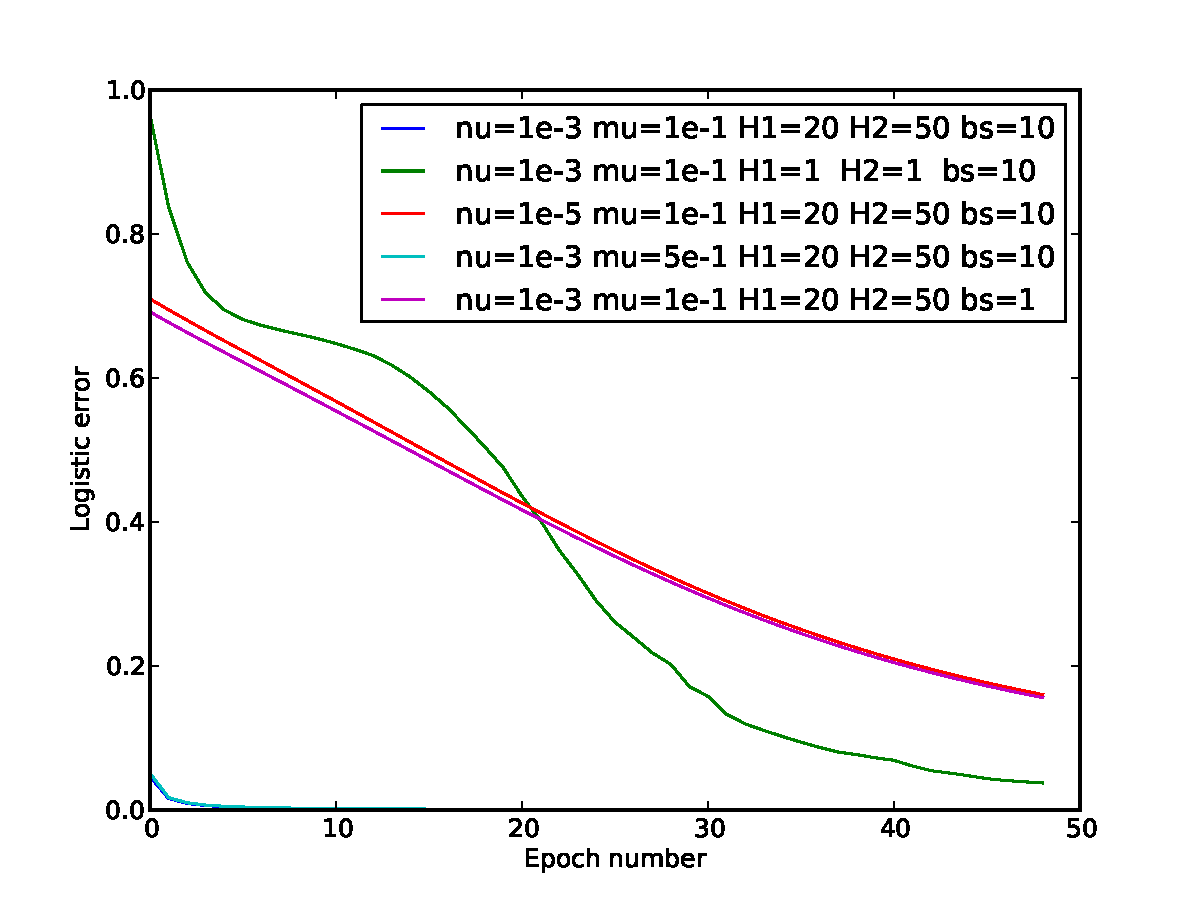
\includegraphics[width=1\columnwidth]{comparative_mlp2}
\par\end{centering}

}%
\end{minipage}\hfill{}%
\begin{minipage}[t]{0.45\columnwidth}%
\subfloat[Example of overfitting for the multi-way MLP used for early-stopping\label{fig:Example-of-overfitting}]{\begin{centering}
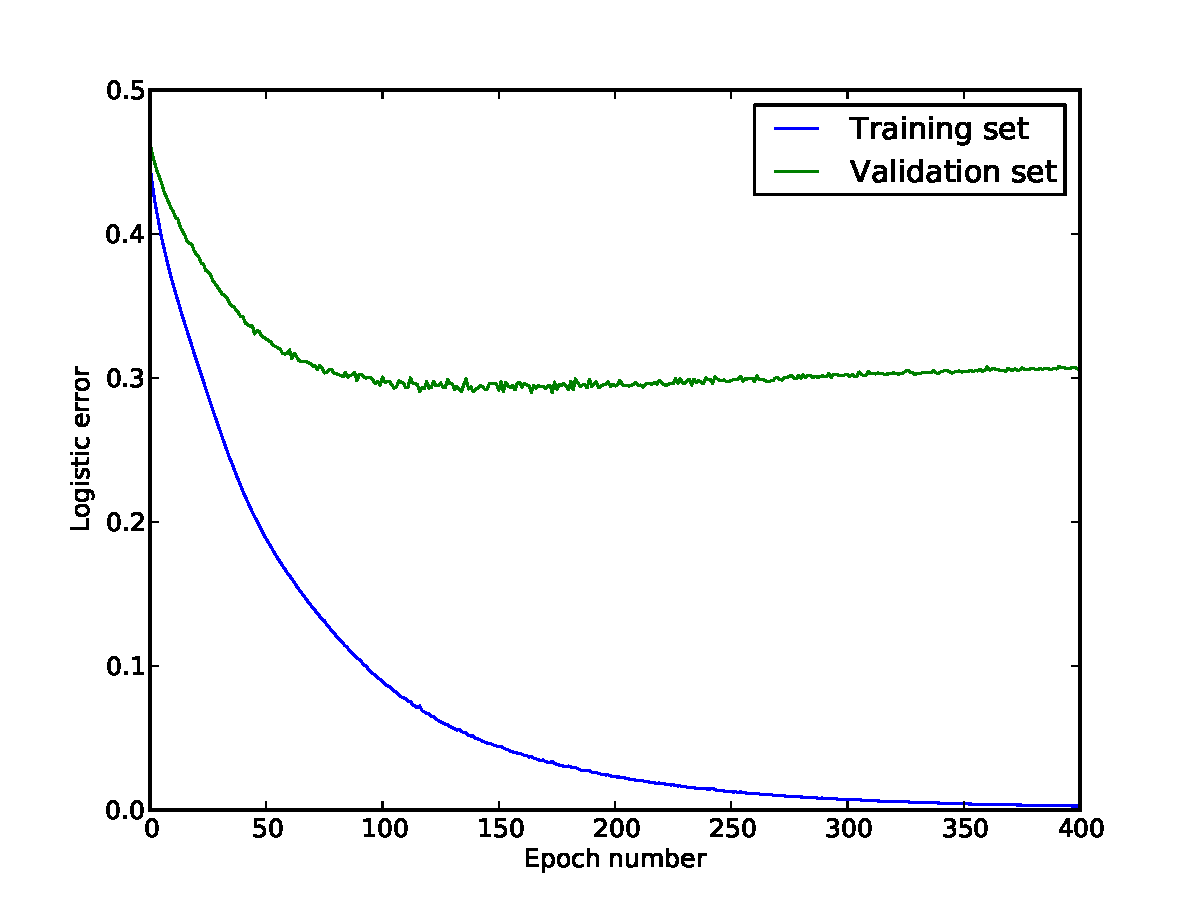
\includegraphics[width=1\columnwidth]{errors_mlp5_overfitting}
\par\end{centering}

}%
\end{minipage}

\caption{MLP training plots}


\end{figure}


Our MLP classifier had two native parameters (namely $H_{1}$ and
$H_{2}$ which we considered separately to ensure analysis completeness),
and relies on gradient descent to converge to the optimal solution,
which adds learning rate $\eta$, momentum term $\mu$ and mini-batch
size to the parameter list. The impact of each parameter on the final
performance of the MLP is unfortunately extremely unintuitive and
difficult to predict, especially because plausible ranges are highly
inter-dependent. Because of this, we couldn't perform standard model
selection by computing errors on the cartesian product of a reasonable
range of parameter values.

We circumvented the problem by running the algorithm with reduced
training and validation sets on a large combinations of values to
get a reasonable estimation. This enabled us to narrow down the search
space and perform better tests with the full training set. See Figure
\ref{fig:Comparative-plot-showing} for examples of how the parameters
influences the convergence of the MLP. For the learning rate $\eta$
we tested with constant values (in the order of $10^{-2}$ to $10^{-5}$)
as well as variations of $10^{-n}x^{-\frac{1}{a}}$ with $n\in\left[0;3\right]$
and $a\in\left[1;3\right]$. The momentum term varied from $0.05$
to $0.25$, and the mini-batch size ranged from $1$ to $50$. As
explained in the problem statement, we tested configuration of MLP
with $1$ to $80$ activation units in each hidden layers.

The optimal parameters for the binary MLP are $\eta=10^{-3}$, $\mu=10^{-1}$,
with mini-batch size of $20$. The numbers of units in the first layer
is $20$ and for the second layer is $50$. For the multi-way MLP,
we found $\eta=10^{-3}$, $\mu=10^{-1}$, mini-batch size of $5$,
and number of units in the first and second layer of $60$ and $10$
respectively.

In Figure \ref{fig:Example-of-overfitting} is an example of overfitting
where the error on the validation set initially decreases but starts
to increase as soon as the MLP is overfitting the training data. We
used early stopping to avoid this behavior in all our gradient-descent
based algorithms.


\subsection{Logistic regression}

The logistic regression technique doesn't have any model parameters,
but it relies on gradient descent which does (namely the learning
rate $\eta$, momentum term $\mu$, and mini batch size). Unfortunately,
as in the MLP case, it is difficult to perform standard model selection
on these parameters.

After having manually determined plausible parameter combinations,
we performed model selection by comparing convergence speed and final
error rate on these values. During this process, we realized that
logistic regression was extremely sensitive to initialization and
training order, so we ran our model selection multiple times on each
parameter combination and considered mean, best case and worst case
performance instead of individual results when comparing models (see
Figure \ref{fig:comparative-logistic}), resulting in the optimal
configuration of $\eta=2e^{-2}$, $\mu=5e^{-2}$, with block size
of $5$.

\begin{figure}[h]
\begin{centering}
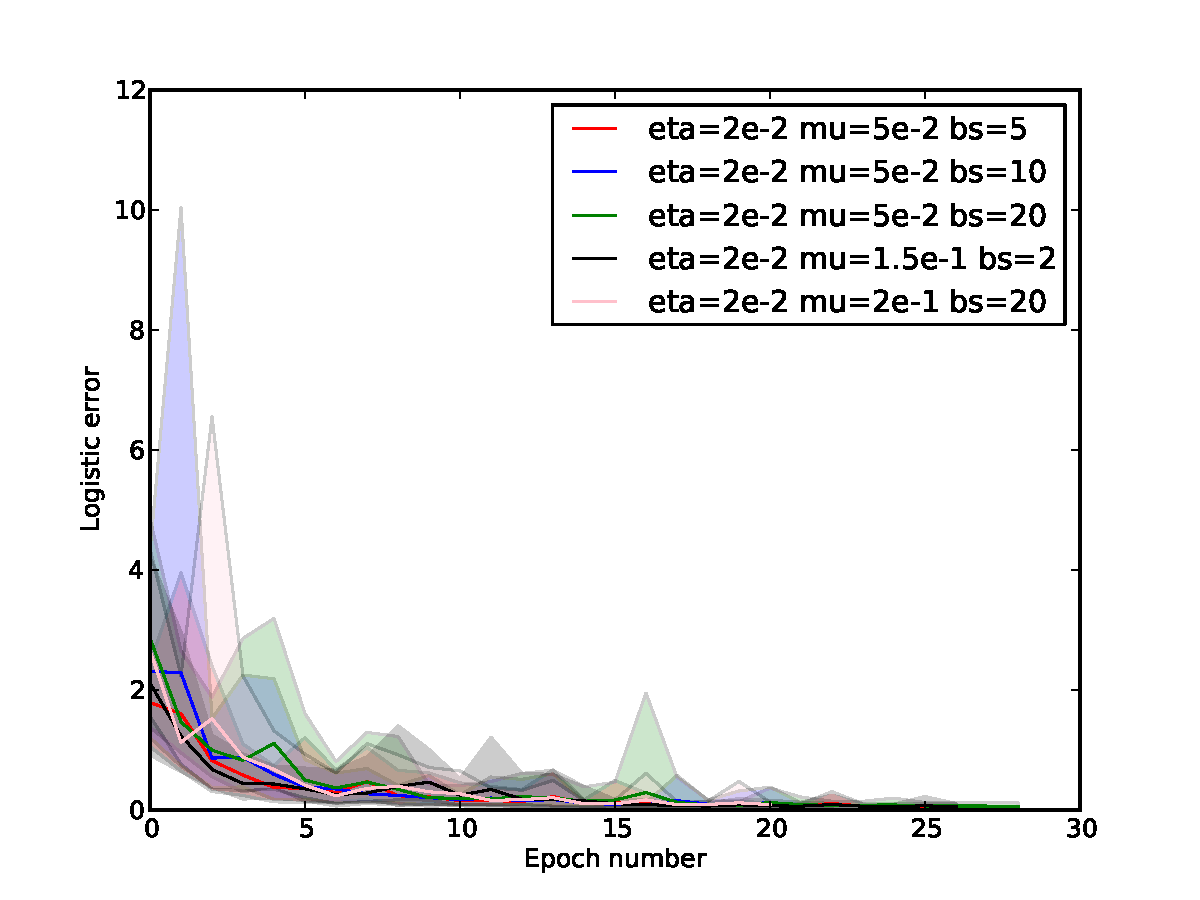
\includegraphics[width=1\columnwidth]{logistic_selection}
\par\end{centering}

\caption{Comparative plot of promising logistic regression model parameter
combinations. The red and black curves both show good initial convergence
and stability, but the red performs better in the tail. \label{fig:comparative-logistic}}


\end{figure}



\subsection{Least squares estimation}


\paragraph{Error function}

The analytical solution to the least squares estimation with Tikhonov
regularization problem is obtained by solving the normal equations
problem. In the case of multi-way classification, the solution is
trivially extended by solving the equations for each of the k vectors
obtained by using \emph{1 of K} encoding for the target vector \textbf{\emph{t}}.
But this also means we multiply the impact of the Tikhonov regularizer
by k. To compensate for this, we modified the regularized error function
slightly :
\[
E(\mathbf{W})=\frac{1}{2}\sum_{i=1}^{N}\parallel\mathbf{y}(\mathbf{x}_{i})-\mathbf{\tilde{t}}_{i}\parallel^{2}+\frac{1}{k}\frac{\nu}{2}\sum_{k=1}^{K}\parallel\mathbf{w}_{k}\parallel^{2}
\]



\paragraph{Model selection}

The model selection process for the least squares estimation technique
was by far the simplest since we were dealing with a single parameter
and a constant convergence time. All computations were performed using
10-fold cross-validation, so we combined the 10 values obtained after
each parameter validation run into boxplots for clarity.

\begin{figure}[h]
\begin{centering}
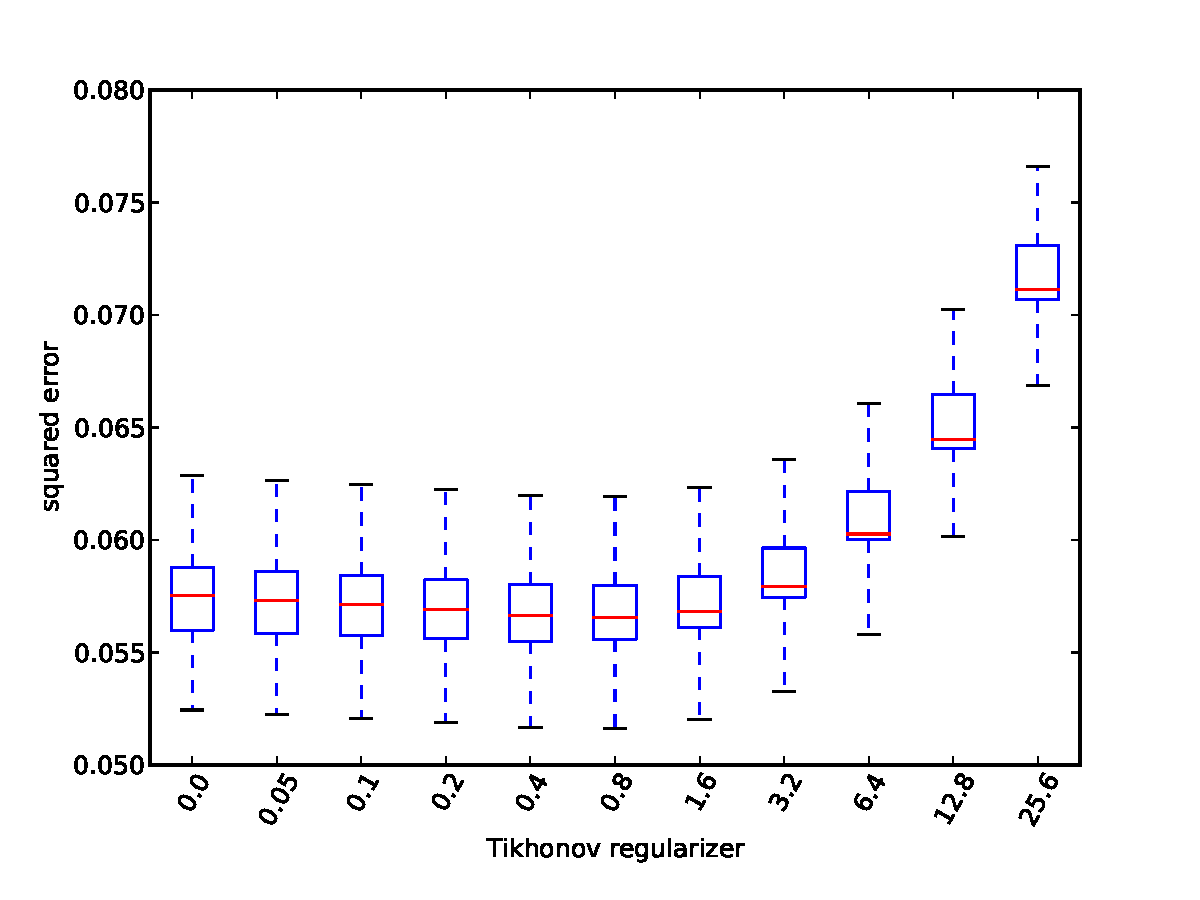
\includegraphics[width=0.8\columnwidth]{lstsq_interval}
\par\end{centering}

\caption{Interval selection for Tikhonov regularization parameter. \label{fig:Interval-selection-lstsq}}
\end{figure}


We initially got a feeling for plausible values by setting the Tikhonov
regularizer to the exponential range $\left\{ 0\right\} \cup\left\{ 5\cdot10^{-2}*2^{k}\mid0\leq k<10\right\} $
(see Figure \ref{fig:Interval-selection-lstsq}). Once we had singled
out a suitable interval, namely $\left[0;1.2\right]$, we performed
a more precise search by resorting to a linear parameter space of
$\left\{ 5\cdot10^{-2}*k\mid0\leq k<25\right\} $ (see Figure \ref{fig:Error-function-value})
and we can thus place the optimal regularizer at $0.6$.

\begin{figure}[h]
\begin{centering}
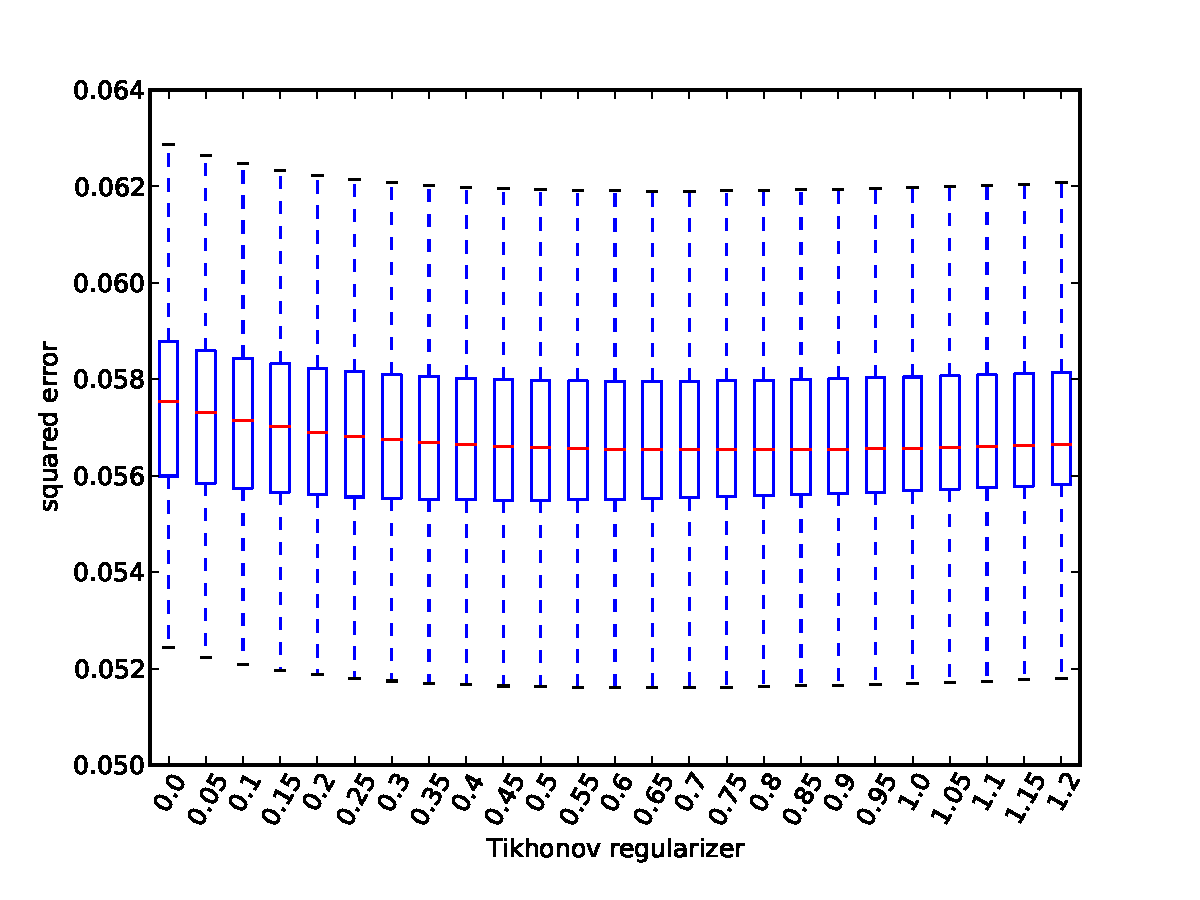
\includegraphics[width=0.5\columnwidth]{lstsq_errors}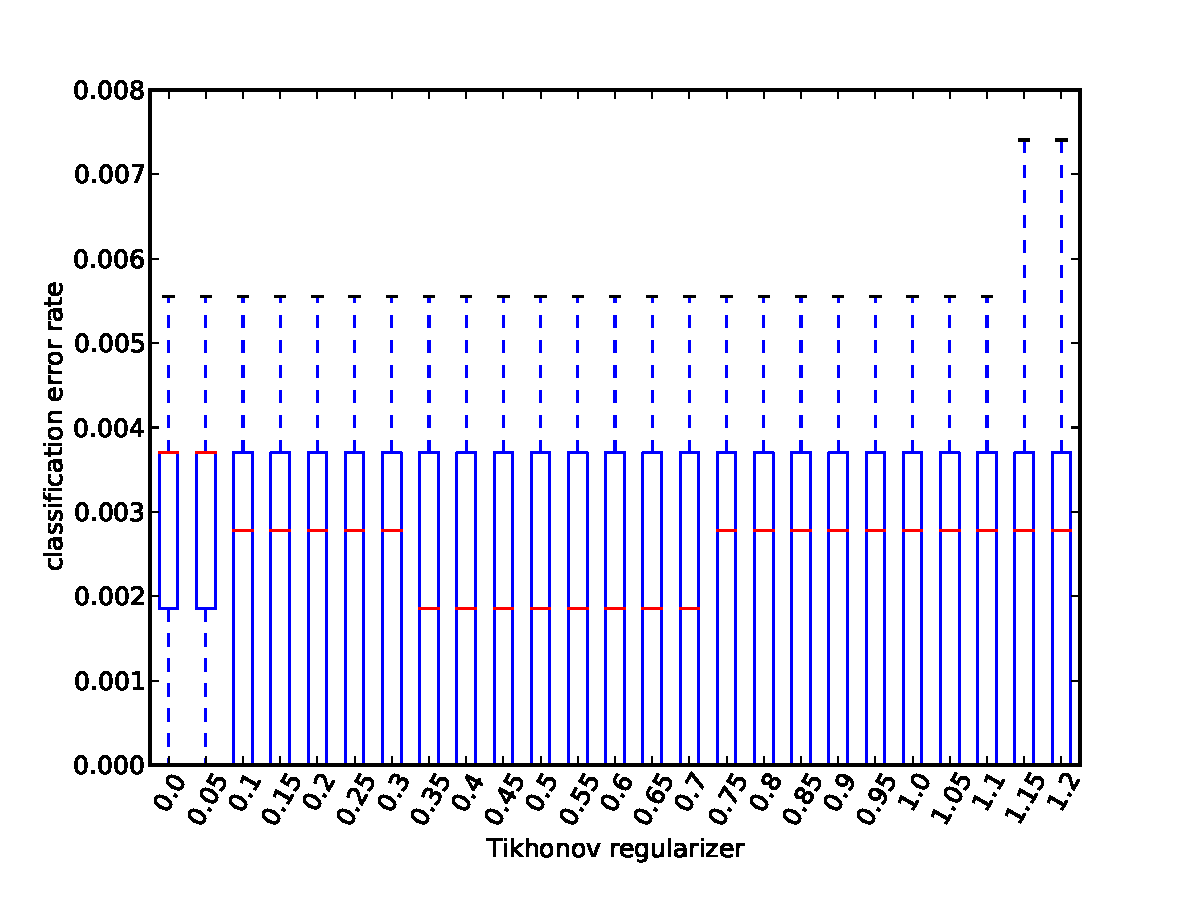
\includegraphics[width=0.5\columnwidth]{lstsq_classerrors}
\par\end{centering}

\caption{Error function value (left) and classification error rate (right)
during parameter selection for Tikhonov regularizer. We can clearly
see the curve minimum around 0.5 (the actual minimum is at 0.6). \label{fig:Error-function-value}}


\end{figure}



\section{Results and Discussion}


\subsection{Binary MLP and multi-way MLP}

\begin{figure}[h]
\begin{centering}
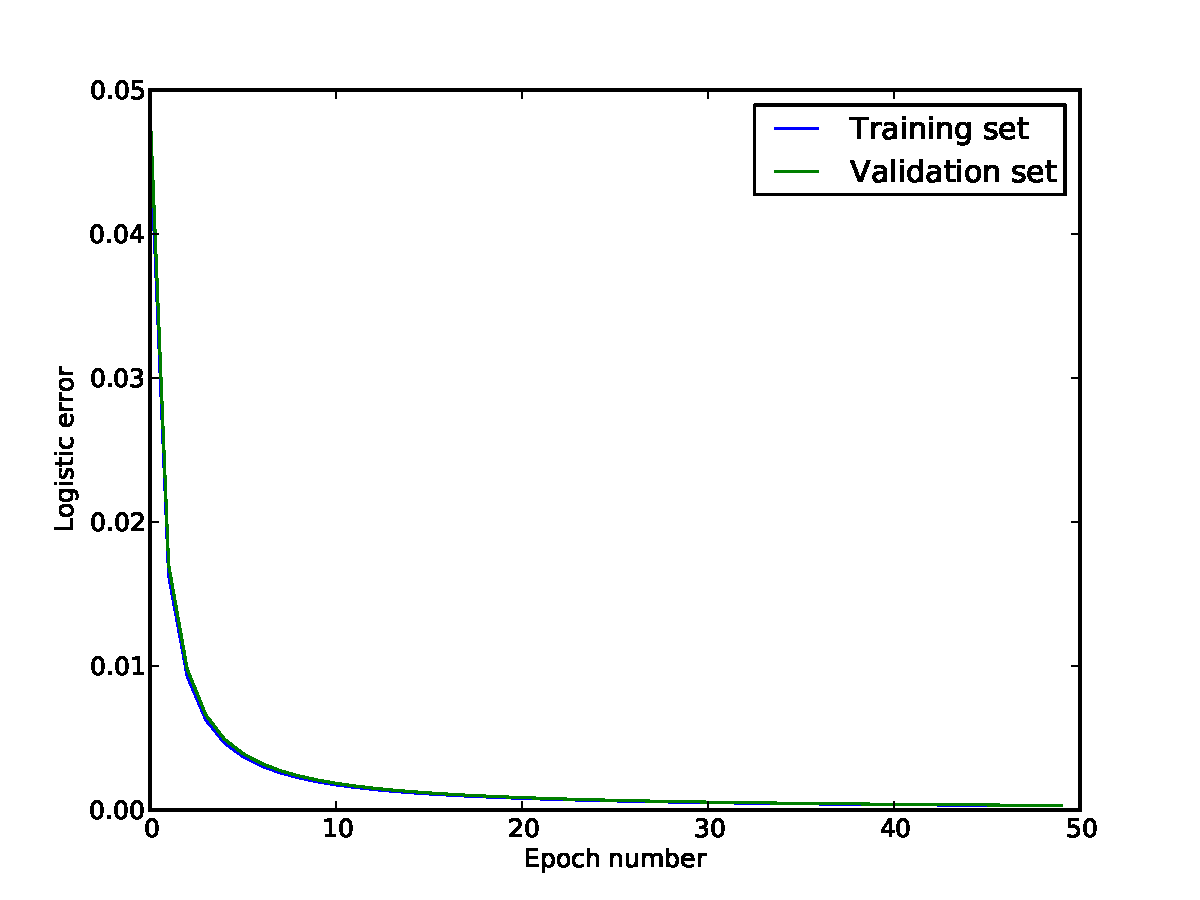
\includegraphics[width=0.8\columnwidth]{errors_mlp2}
\par\end{centering}

\caption{Logistic error for binary classification using MLP for the training
and the validation set. The classification error rate is not very
interesting in this setting since it drops to zero after one run over
all training points. \label{fig:Logistic-error-for}}
\end{figure}


The graph in Figure \ref{fig:Logistic-error-for} shows the logistic
error computed with the optimal parameters for the binary MLP. Both
the errors for the training and validation sets are very close and
the MLP converges quickly to an optimal solution, as both the classification
error for the training and the validation set are null.

\begin{figure}[h]
\begin{centering}
\subfloat[]{\begin{centering}
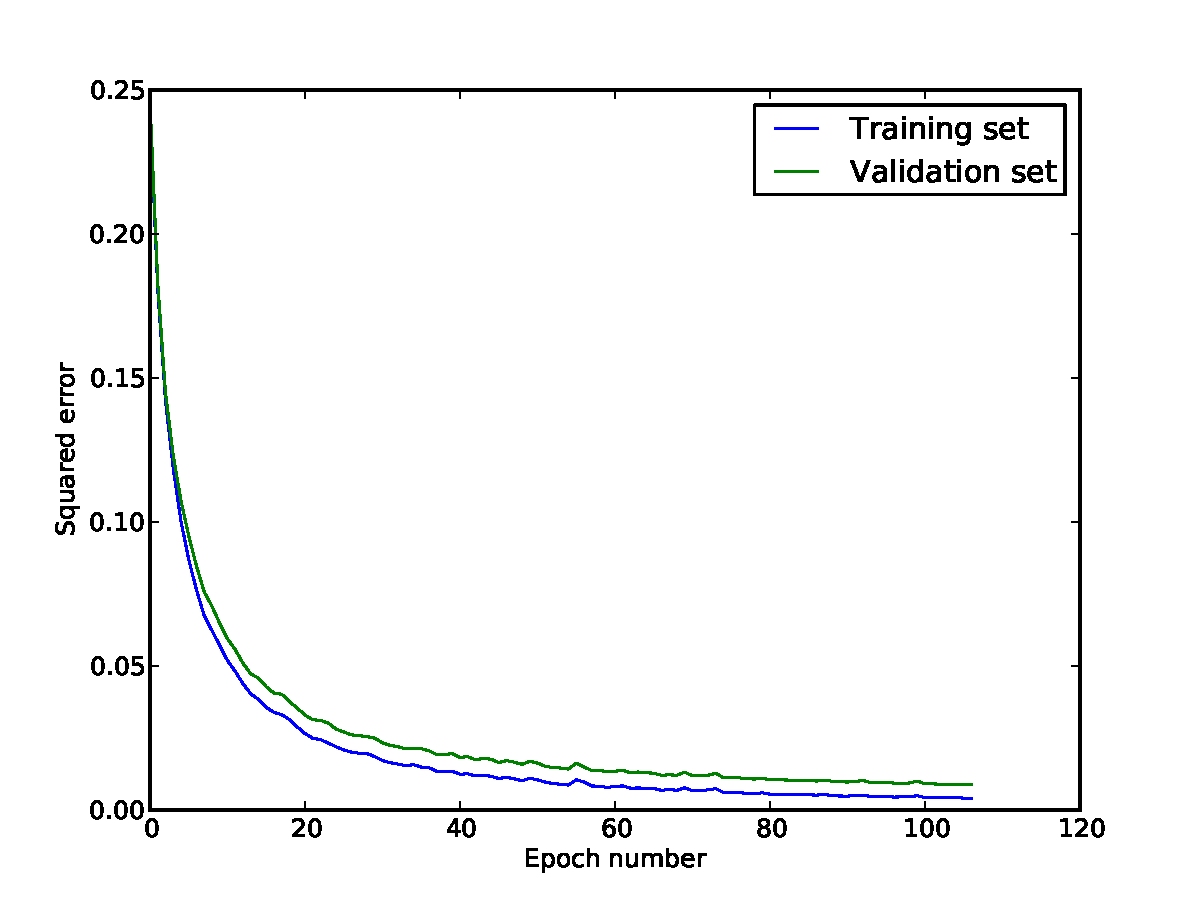
\includegraphics[width=0.5\columnwidth]{errors_mlp5}
\par\end{centering}

}\subfloat[]{\begin{centering}
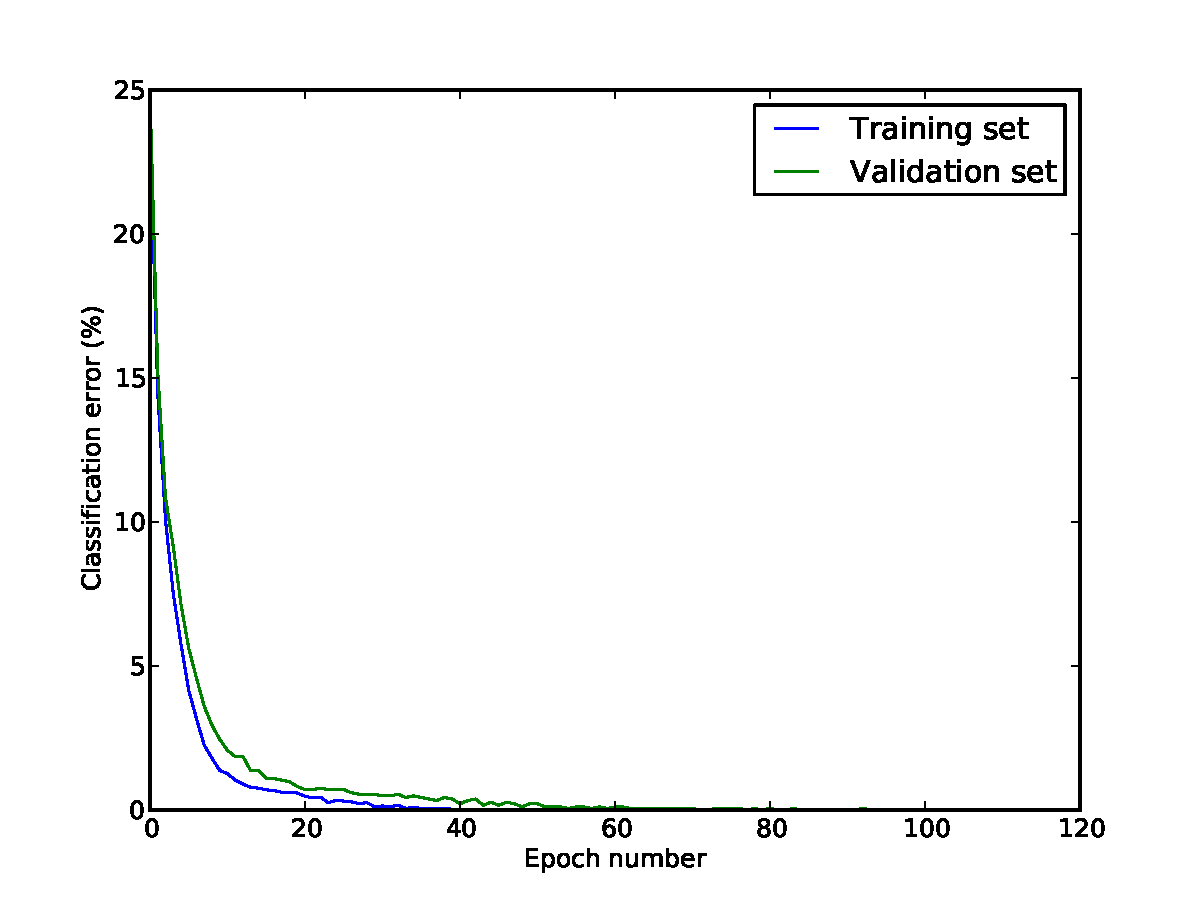
\includegraphics[width=0.5\columnwidth]{classerrors_mlp5}
\par\end{centering}



}
\par\end{centering}

\caption{Squared error (a) and classification error (b) for multi-way classification
using MLP for the training and the validation set.\label{fig:Logistic-error-for-1}}
\end{figure}


The graph in Figure \ref{fig:Logistic-error-for-1} shows the same
metric for the multi-way MLP. The system converges slower than before
and there is a better separation between the errors of the training
and the validation set. We also showed a graph representing the classification
error for both sets, as they both converge to zero but not at the
same speed. It is interesting to notice that both the binary and multi-way
MLP converge to a classification error of zero after enough training.


\subsection{Logistic regression}

In Figure \ref{fig:Logistic-error-for-1-1}, we show the error for
the logistic regression technique in function of the training epoch.
We see right away that the convergence speed is close to the one we
witnessed in the MLP case, but the classification error rate of the
validation set is much lower using the multi-way MLP technique.

\begin{figure}[h]
\begin{centering}
\subfloat[]{\begin{centering}
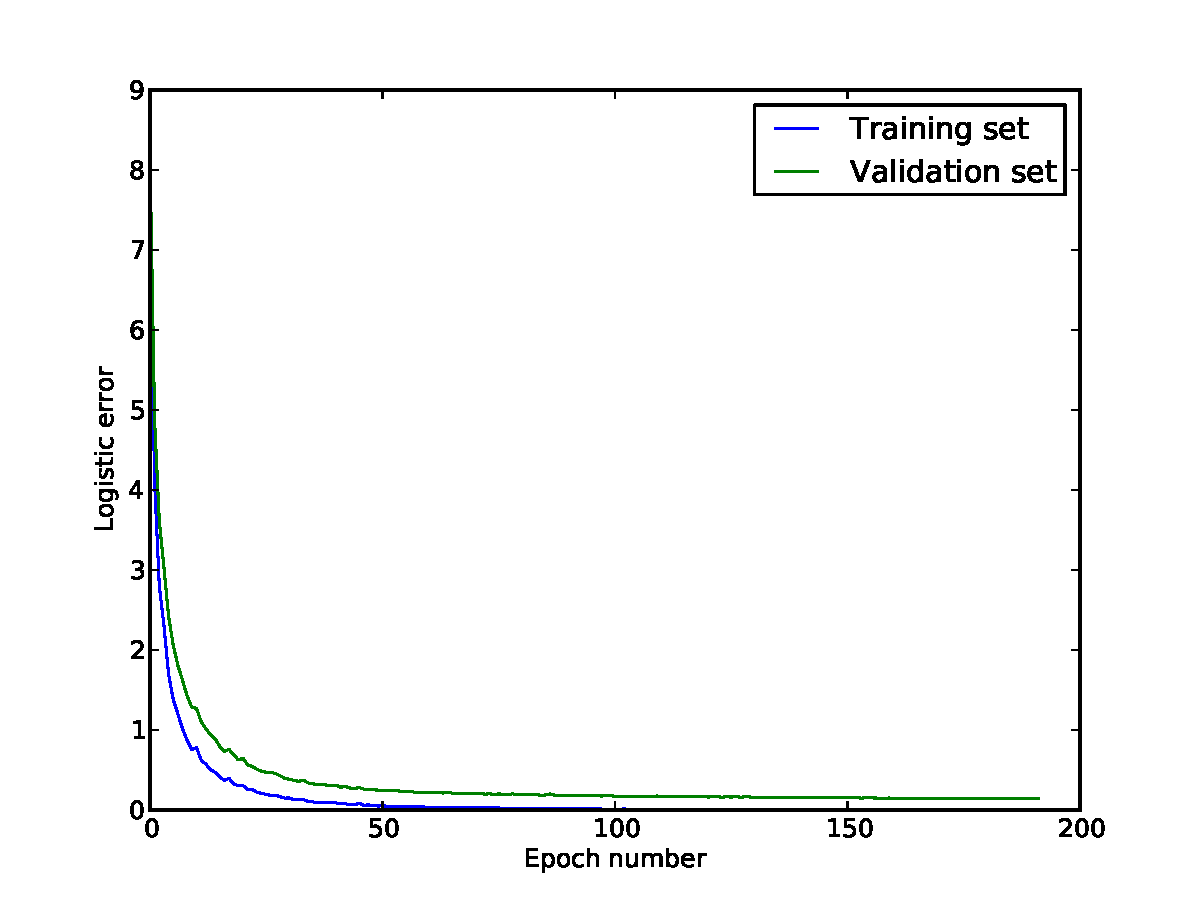
\includegraphics[width=0.5\columnwidth]{errors_logistic}
\par\end{centering}

}\subfloat[]{\begin{centering}
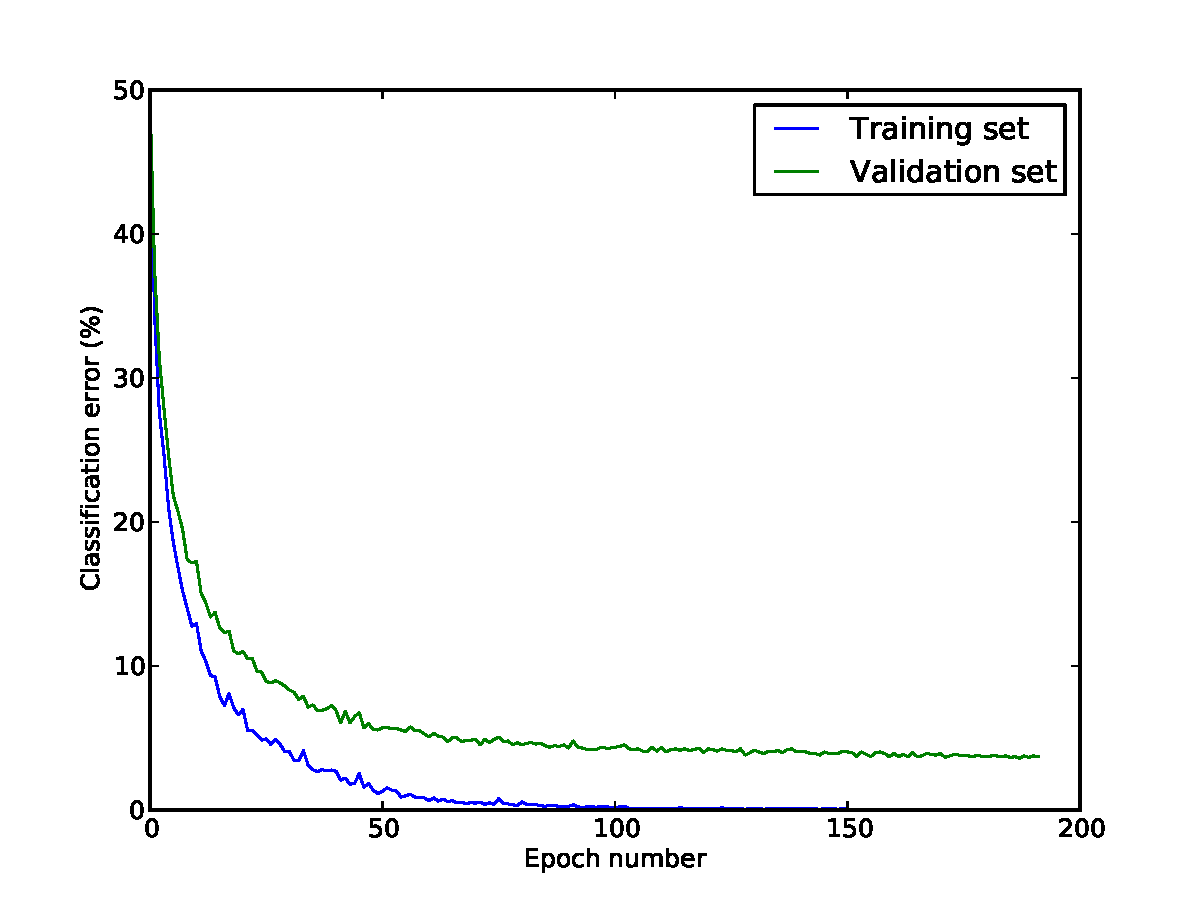
\includegraphics[width=0.5\columnwidth]{classerrors_logistic}
\par\end{centering}

}
\par\end{centering}

\caption{Logistic error (a) and classification error (b) for multi-way classification
using logistic regression for the training and the validation set.\label{fig:Logistic-error-for-1-1}}
\end{figure}



\subsection{Classification results}

\begin{figure}[h]
\begin{centering}
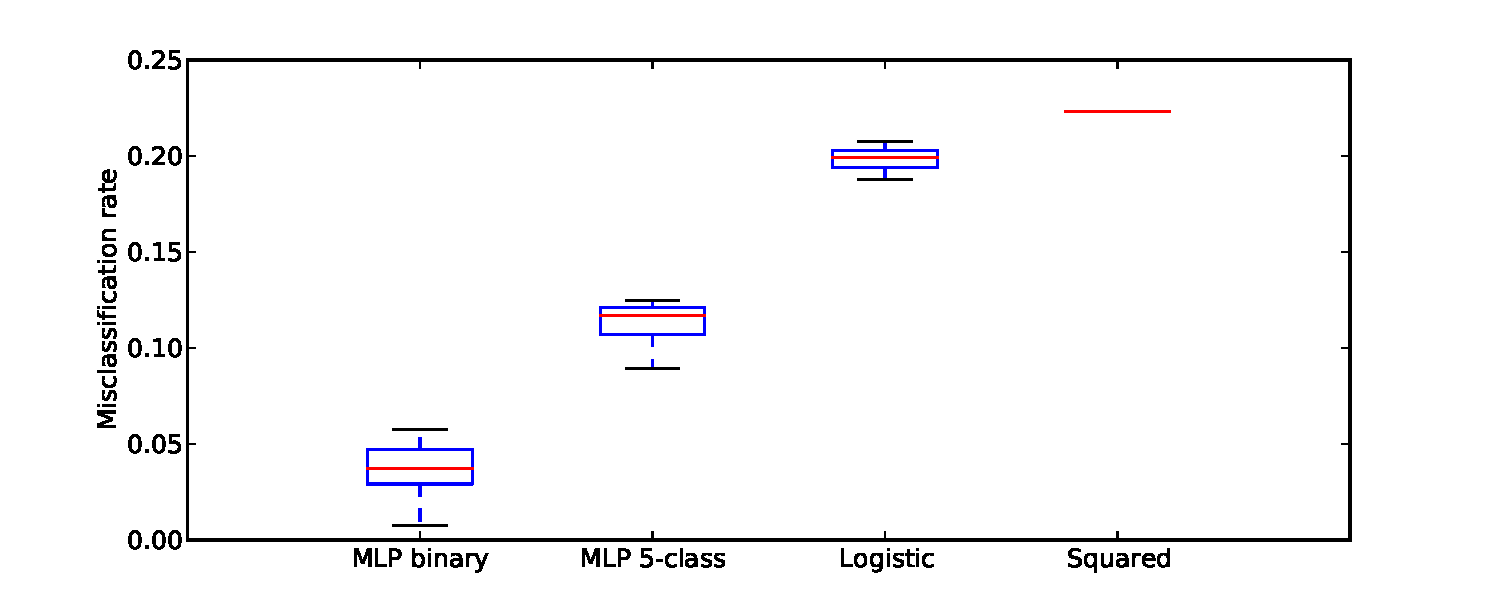
\includegraphics[width=0.8\columnwidth]{testing_boxplot}
\par\end{centering}

\caption{Comparative boxplot for each classifier\label{fig:Comparative-boxplot-for}}
\end{figure}


The results for the misclassification rate on the test set are shown
in Figure \ref{fig:Comparative-boxplot-for}. Both implementations
of MLP show higher performance than linear classifiers. On the binary
classification dataset, the binary MLP misclassified $\mathbf{3.65}\%$(\textbf{$\sigma=1.37$}).
On the 5-way classification dataset, the MLP had an average error
percentage of \textbf{$\mathbf{11.29}\%$} ($\sigma=1.11$), the logistic
regression performed worse with an average of \textbf{$\mathbf{19.84}\%$}
($\sigma=0.61$) classification errors. All those results were computed
on 10 runs. Linear regression with squared error had the worse classification
error percentage with $\mathbf{22.34}\%$.

\begin{figure}[h]
\subfloat[Binary MLP]{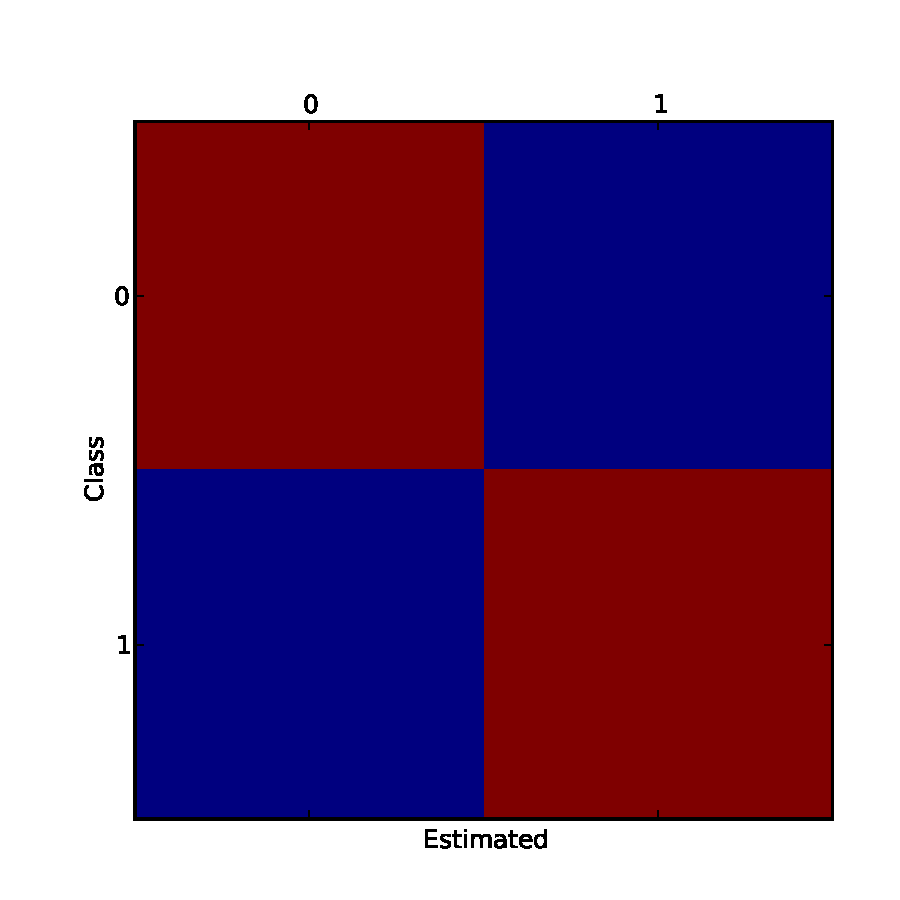
\includegraphics[width=0.25\columnwidth]{confusion_mlp2}



}\subfloat[Multi-way MLP]{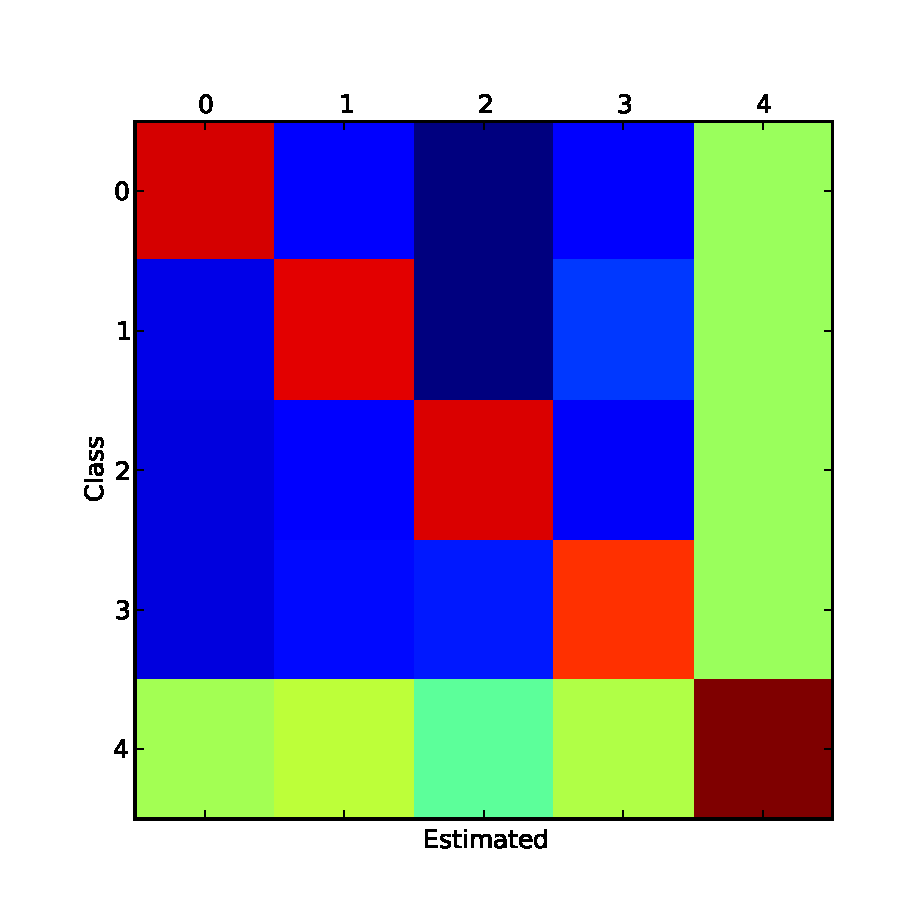
\includegraphics[width=0.25\columnwidth]{confusion_mlp5}

}\subfloat[Logistic error regression]{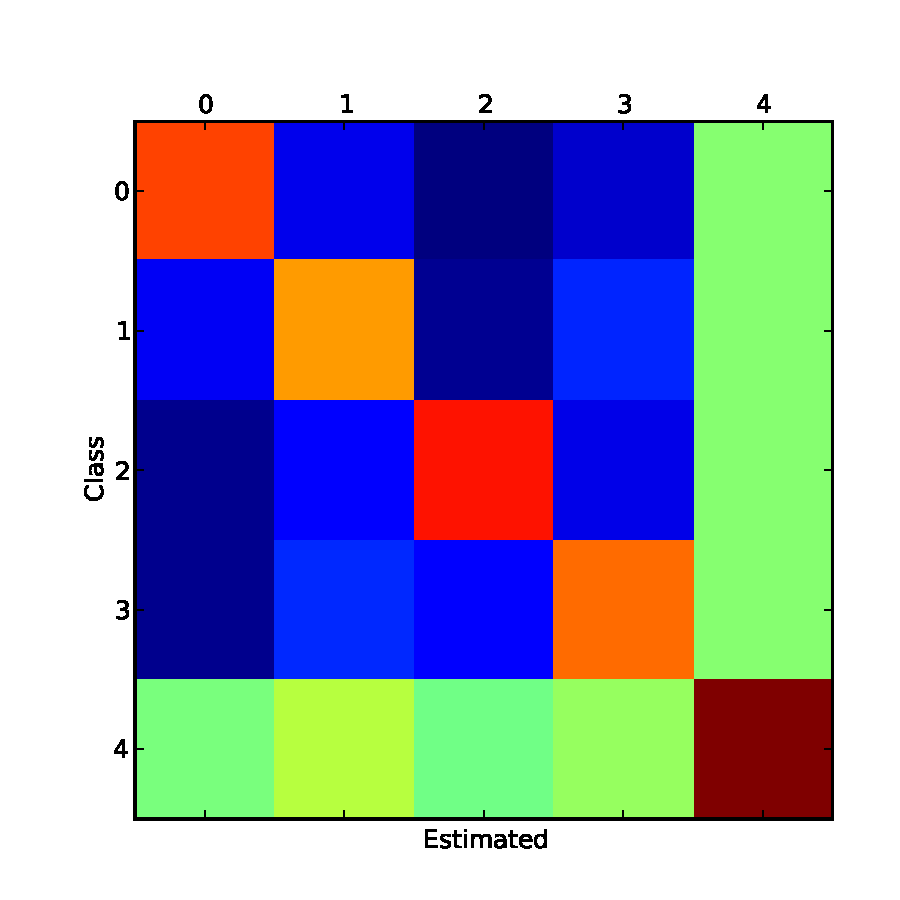
\includegraphics[width=0.25\columnwidth]{confusion_logistic} 

}\subfloat[Squared error regression]{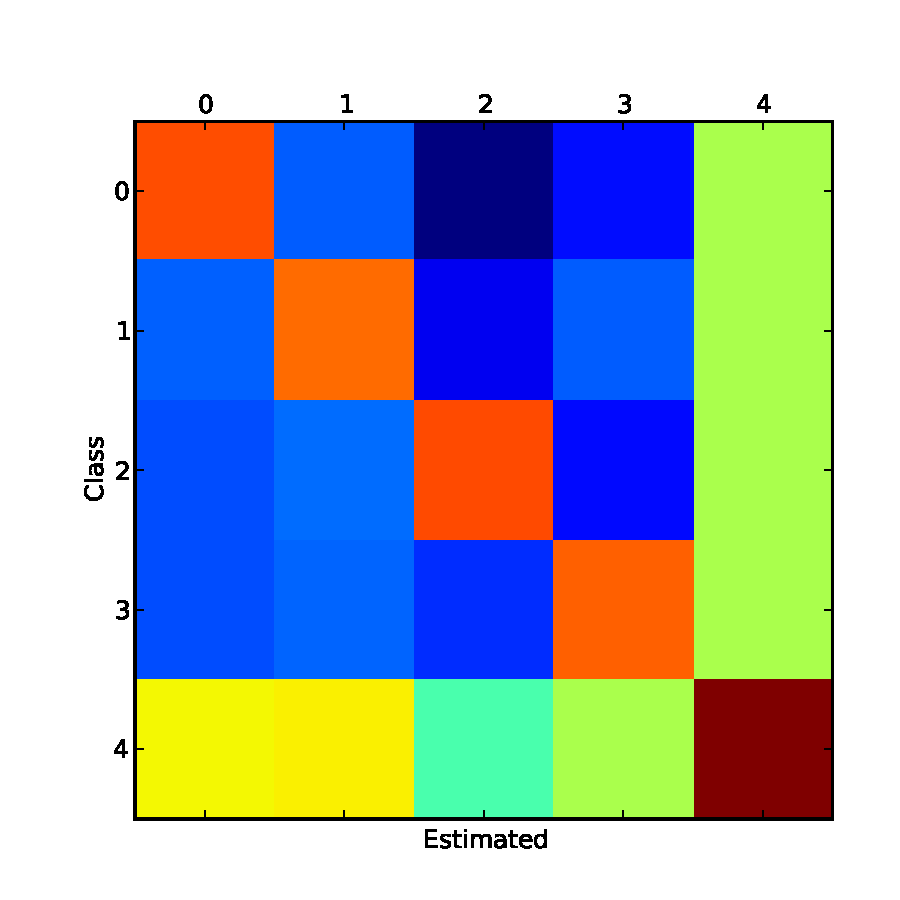
\includegraphics[width=0.25\columnwidth]{confusion_lstsq}

}

\caption{Confusion matrices (qualitative comparison)\label{fig:Confusion-matrices}}
\end{figure}


The confusion matrices are shown in Figure \ref{fig:Confusion-matrices}.
As expected and confirmed by the boxplot in Figure \ref{fig:Comparative-boxplot-for},
the binary MLP performs very well with very few errors. The multi-class
classification methods are more confused by the input images as the
classes are closer to each other in terms of feature space. This qualitative
comparison shows a decay in classification performance from the MLP
to the squared error regression, confirming the results of Figure
\ref{fig:Comparative-boxplot-for}.

\begin{figure}[h]
\begin{centering}
\subfloat[Negative $t_{i}a_{i}^{\left(3\right)}$ close to zero]{
\includegraphics[scale=4]{bad_left}
\includegraphics[scale=4]{bad_right}



}\subfloat[Large negative $t_{i}a_{i}^{\left(3\right)}$]{
\includegraphics[scale=4]{verybad_left}
\includegraphics[scale=4]{verybad_right}

}\caption{Misclassified image examples with the multi-way MLP}

\par\end{centering}

\end{figure}

\end{document}
